\svnInfo $Id: praxis.tex 75 2008-04-07 13:37:13Z axel $
\chapter{Praxis}

Im ersten Abschnitt dieses Kapitels wird kurz auf die Erfahrungen eingegangen, die während der Analyse und Implementierung einiger der beschriebenen Verfahren gemacht wurden. Darauf folgt eine knappe Einführung in die Struktur der erstellten Software.

\label{chap:fazit}
\section{Implementierung}

Die im Zusammenhang mit dieser Arbeit erstellte Anwendung unterstützt als Objekte der Szene lediglich Dreiecke. Damit folgt sie den Implementierungen vieler aktueller Realtime Raytracer (\cite{Wald04}, \cite{Waechter08}). Prinzipiell ermöglicht der allgemeine Raytracing Algorithmus die Verwendung beliebiger Objekte, für die ein Strahlschnittest zur Verfügung steht. Die verschiedenen Strahlschnitttests müssten jedoch mit in den Traversierungsalgorithmus aufgenommen werden. Die entsprechende Vergößerung dieses Codeabschnitts, in Verbindung mit den datenabhängigen Sprüngen für die Schnittests, würden eine signifikante Verschlechterung der Gesamtleistung bewirken.

Für die erste Implementierung konnten interaktive Frameraten lediglich für mittlere bis kleine Szenen erreicht werden (<50k Dreicke). Daraufhin wurde von einer weiteren Optimierung des Codes abgesehen, da dies die Lesbarkeit weiter herabgesetzt hätte und die Leistungsfähigkeit der vorgestellten Algorithmen bereits von den Autoren demonstriert wurde.
Anstatt dessen wurde die Architektur zugunsten einer leicht verständlichen Struktur umgestaltet. Für die Anwendung können viele Parameter, wie zum Beispiel die verwendete Beschleunigungsdatenstruktur, zur Laufzeit konfiguriert werden.
Die implementierte Struktur ermöglicht die einfache Implementierung weiterer Verfahren.

Einige der vorgestellten Verfahren sind sowohl in einer leicht verständlichen (zum Beispiel rekursiven) als auch in einer effizienteren Variante (kompakte Speicherauslegung, iterative Traversierung) implementiert. Um die Lesbarkeit beizubehalten wurden einige Kompromisse eingegangen. So wird zum Beispiel auch in häufig ausgeführtem Code, nicht gänzlich auf die Verwendung virtueller Methoden verzichtet.

Die im Zusammenhang mit der Arbeit erstellte Codebasis soll nicht als Leistungsdemonstration der Verfahren dienen, sondern vielmehr Einblick in die verschiedenen Verfahren zur Raumaufteilung geben. Zusätzlich soll durch die Möglichkeit, naive mit optimierten Implementierungen direkt zu vergleichen, veranschaulicht werden, welche Änderungen für die Verwendung bestimmter Techniken und Technologien am Code vorgenommen werden müssen.

\section{Programmstruktur}

Die Quelldateien der Software sind in folgende Unterverzeichnisse gegliedert:
\begin{description}
 \item[acceleration]Das Verzeichnis enthält alle Klassen, die Beschleunigungsdatenstrukturen umsetzen oder ausschließlich von diesen genutzt werden.
 \item[core]Geometrische Primitive sowie weitere Klassen, die für die Konstruktion eines Raytracers nötig sind, werden hier abgelegt.
 \item[renderer]Unabhängig von den Beschleunigungsstrukturen lassen sich verschiedene Strategien für die finale
 Bildsynthese wählen (einzelne Strahlen, Pakete etc.). Die unterschiedlichen Strategien werden in \textit{Renderern} gekapselt, die in diesem Verzeichnis zu finden sind.
 \item[shader]Im \textit{shader}-Verzeichnis befinden sich die Klassen, die das unterschiedliche Verhalten von Materialien beim Auftreffen von Licht implementieren.
 \end{description}

Diagramm \ref{fig:basicuml} zeigt das Zusammenspiel der wichtigsten Klassen. Die Klasse \\ \verb|AccellerationStructure| bildet die Schnittstelle für die verschiedenen Beschleunigungsdatenstrukturen. Die drei Methoden außer \verb|construct()| dienen der Beantwortung der in Kapitel \ref{chap:rt} vorgestellten drei Problemen. Neben den gezeigten enthält die Schnittstelle auch die Signaturen für die Beantwortung dieser Probleme für mehrer Strahlen gleichzeitig mit Unterstrützung des SSE Befehlssatzes.

\verb|AccellerationStructure| wird von folgenden Klassen implementiert
\begin{description}
 \item[PrimitiveList]Implementiert den in Abschnitt \ref{sec:naiv} beschriebenen naiven Ansatz ohne jegliche Beschleunigung
 \item[RegularGrid]Ein gleichmäßiges Gitter welches den in Kapitel \ref{sec:fastgrid} beschriebenen Algorithmus zur Traversierung nutzt.
 \item[KdTreeSimple]Zeigt eine unoptimierte Version des kd-Trees zu Ver\-deut\-lich\-ung der grund\-sätz\-lich\-en Funktionsweise.
 \item[KdTreeBase]Oberklasse für verschiedene kd-Tree Varianten, die alle die in Abschnitt \ref{sec:toxiememlayout} beschriebene Speicherauslegung verwenden.
\begin{description}
 \item[KdTreeSAHNaive]Implementiert den naiven Ansatz zur Konstruktion mit der SAH mit $O(n^2)$
 \item[KdTreeSahNlog2N]Implementiert den in Abschnitt \ref{sec:nlog2n} vorgestellten Algorithmus zur Konstruktion mit $O(n {log}^2n)$.
\item[KdTreeSahNlogN]Konstruiert den kd-tree mit $O(n {log} n)$ wie in Abschnitt \ref{sec:nlog2n} beschrieben.
 \end{description}
\item[Bih]Nicht optimierte Version der BIH, zur Veranschaulichung der allgemeinen Vorgehensweise
\item[BihCompact]Verwendet die kompakte Speicherauslegung für BIH-Knoten
\item[BihIterative]Verwendet die kompakte Speicherauslegung und traversiert die Hierarchie iterativ
 \end{description}

Die Shader dienen dazu, für einen Punkt der Szenengeometrie zu ermitteln, wieviel Licht von dort in eine bestimmte Richtung reflektiert wird. Die Klasse \verb|Shader| definiert hierzu zwei Signaturen, eine für einzelne Punkte und eine für mehrere Punkte im SIMD Format. Zur Zeit sind drei einfache Shader implementiert:
\begin{description}
 \item[FlatShader]gibt immer einen konstanten Farbwert zurück
 \item[DirectShader]berechnet den reflektierten Anteil des Lichts der direkt von den Lichtquellen abgegeben wird
 \item[SpecularShader]berechnet die Anteile, die durch perfekte Reflektion und Transmission in die gegebene Richtung abgegeben werden.
 \end{description}

\begin{figure}\centering
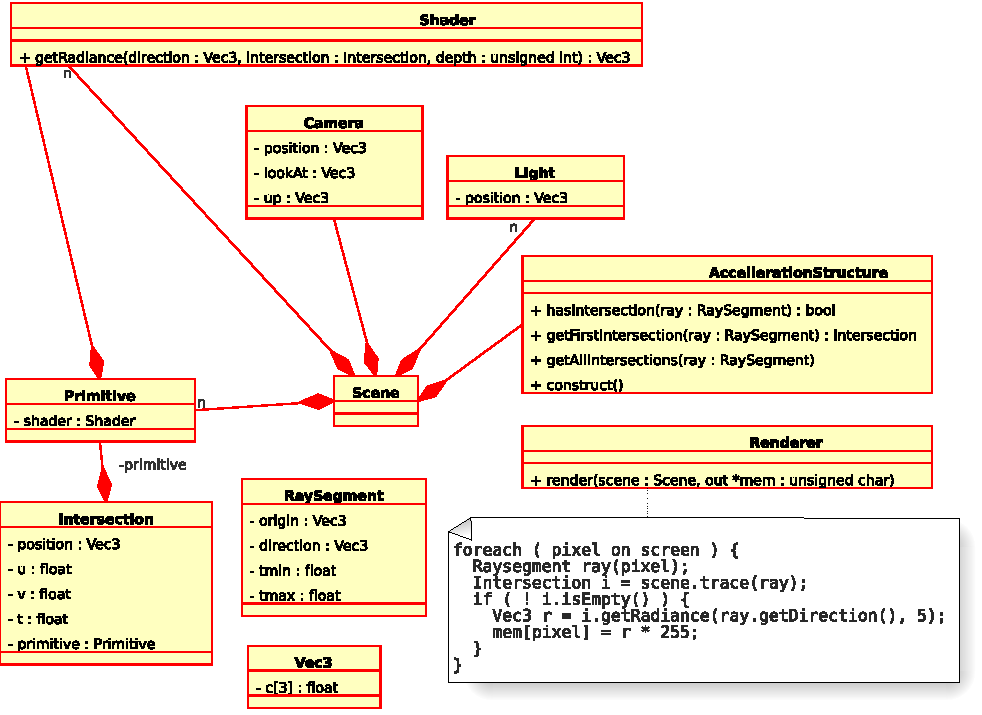
\includegraphics[width=1.0\textwidth]{images/basicuml.pdf} 
\caption[Diagramm der wichtigsten Klassen]{Das Diagramm zeigt nicht alle Details der Implementierung. Der Codeschnipsel rechts unten zeigt den prinzipiellen Ablauf des Renderings eines Bilds. Der entrsprechende C++-Code zum gezeigten Pseudocode finde sich in der Klasse SingleRayRenderer wieder.}
\label{fig:basicuml}
\end{figure}

\chapter{Fazit}

Raytracing allgemein ist ein Forschungsgebiet auf dem seit nun fast 30 Jahren geforscht wird. Einsteigern in diesem Gebiet steht deswegen eine umfangreiche, aber nicht immer übersichtliche Menge an Literatur zur Verfügung. Durch die ständig steigende Leistungsfähigkeit der Computer ist das Interesse am Raytracingverfahren, besonders in der Kombination mit echtzeitfähigen Algorithmen, in den letzten Jahren stark angestiegen. Dementsprechend ist auch die Anzahl und Frequenz der Veröffentlichungen zu diesem Thema angestiegen.
Die unterschiedlichen Arbeiten sind besonders vor dem Hintergrund dynamischer Szenen oft nur schwer zu bewerten, beziehungsweise zu vergleichen. Hingegen sind sich alle Autoren einig, dass es nicht \textbf{das} beste Verfahren gibt. Zuviele Einflussfaktoren bestimmen die letztendliche Leistung eines Raytracers. Zusätzlich gilt, dass eine für einen bestimmten Anwendungsfall optimierter Lösung immer eine allgemeinere Lösung übertreffen wird.
In dieser Arbeit wurden die drei aktuell konkurrierenden Verfahren zur Raumaufteilung mit ihren Vor- und Nachteilen vorgestellt (Gitter, hierarchische Raumaufteilung, Partitionierung der Objektmenge). Bei der Auswahl eines Verfahrens für einen konkreten Anwendungsfall sollten die Vor- und Nachteile, die sich für die verschiedenen Verfahren aus der Parametern der Anwendung ergeben, genau untersucht werden. Je nach Szenengröße, Art der Dynamik, Verteilung der Objekte usw. kann sich das eine oder das andere Verfahren besser für einen bestimmten Fall eignen.

Die vorgestellten Richtlininen für die Anwendungsentwicklung auf aktueller Hardware gelten allgemein für die Entwicklung leistungsorientierter Anwendungen. Dabei sei noch einmal darauf hingewiesen, dass die Optimierung für beste Cachebenutzung mit Abstand die wichtigste Optimierung darstellt. Für eine ausführliche Erläuterung der Optimierungsmöglichkeiten bei der Anwendungsentwicklung sei auf \cite{Drepper07} und \cite{Fog08} verwiesen.

Unter Umständen wird die Hardwarearchitektur der Rechner in Zukunft soweit optimiert werden, dass Raytracing in Echtzeit auch ohne spezielle Berücksichtigung der Hardware möglich wird. Fakt ist aber, dass auch aktuelle Implementierungen immer noch viele grobe Annäherungen bei der Simulation des Lichtflusses machen. Eine optimierte Anwendung kann die gewonnenen Kapazitäten in die Simulation bisher nur mäßig darstellbarer Phänomene investieren. So stellen zum Beispiel Global Illumination und Distributed Raytracing bisher noch genug Probleme, welche momentan nicht in Echtzeit gelöst werden können, dass auch die Prozessoren kommender Rechnergenerationen, allein mit der Darstellung von 3d-Szenen voll ausgelastet werden können..

Diese Entwicklung deutet zwar darauf hin, dass in Zukunft immer ansprechendere Grafiken, auch in Echtzeit, generiert werden können. Sie zeigt aber auch, dass immer der Bedarf für eine auf aktuelle Hardware optimierte Lösung bestehen wird.